\documentclass{article}
\usepackage{mathrsfs} % for scripts
\usepackage{standalone}
\usepackage{tikz}
\usetikzlibrary{hobby}
\begin{document}
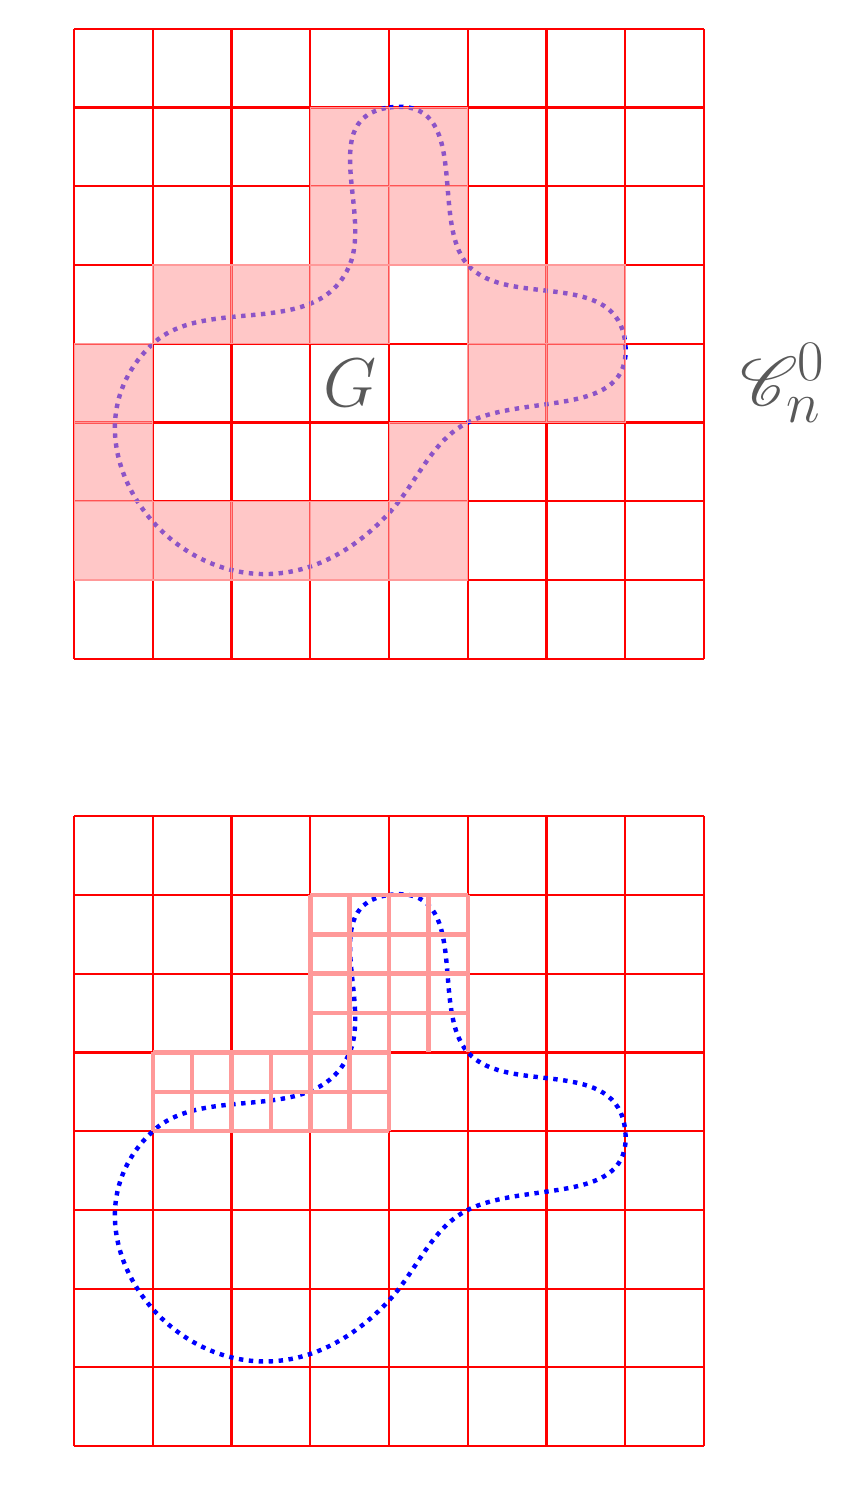
\begin{tikzpicture}
    \begin{scope}[closed hobby,fill opacity=0.65]
	\draw[step=1.0cm,red,thick] (-4,-4) grid (4,4);
	\draw[ultra thick,dotted,blue] plot coordinates {( 0,3)(1,1)(3,0)(1,-1)(0,-2.15)(-3.0,0)
	    (-0.5,1)} ;
	\node at (-0.5,-0.5) {\Huge$G$};
	\node at (5,-0.5) {\Huge$\mathscr{C}_n^0$};
	\filldraw[red!40,fill opacity=0.55] (-1,2) rectangle (0,3);
	\filldraw[red!40,fill opacity=0.55] (-1,1) rectangle (0,2);
	\filldraw[red!40,fill opacity=0.55] (-1,0) rectangle (0,1);
	\filldraw[red!40,fill opacity=0.55] (-2,0) rectangle (-1,1);
	\filldraw[red!40,fill opacity=0.55] (-3,0) rectangle (-2,1);
	%\filldraw[red!40,fill opacity=0.55] (-3,-1) rectangle (-2,0);
	\filldraw[red!40,fill opacity=0.55] (-4,-1) rectangle (-3,0);
	\filldraw[red!40,fill opacity=0.55] (-4,-2) rectangle (-3,-1);
	\filldraw[red!40,fill opacity=0.55] (-4,-3) rectangle (-3,-2);
	\filldraw[red!40,fill opacity=0.55] (-3,-3) rectangle (-2,-2);
	\filldraw[red!40,fill opacity=0.55] (-2,-3) rectangle (-1,-2);
	\filldraw[red!40,fill opacity=0.55] (-1,-3) rectangle (0,-2);
	\filldraw[red!40,fill opacity=0.55] (0,-3) rectangle (1,-2);
	\filldraw[red!40,fill opacity=0.55] (0,-2) rectangle (1,-1);
	\filldraw[red!40,fill opacity=0.55] (1,-1) rectangle (2,0);
	\filldraw[red!40,fill opacity=0.55] (2,-1) rectangle (3,0);
	\filldraw[red!40,fill opacity=0.55] (2,0) rectangle (3,1);
	\filldraw[red!40,fill opacity=0.55] (1,0) rectangle (2,1);
	\filldraw[red!40,fill opacity=0.55] (0,1) rectangle (1,2);
	\filldraw[red!40,fill opacity=0.55] (0,2) rectangle (1,3);
    \end{scope}
    \begin{scope}[yshift=-10cm,closed hobby,fill opacity=0.65]
	\draw[step=1.0cm,red,thick] (-4,-4) grid (4,4);
	\draw[ultra thick,dotted,blue] plot coordinates {( 0,3)(1,1)(3,0)(1,-1)(0,-2.15)(-3.0,0)
	    (-0.5,1)} ;
	\draw[step=0.5,red!40,ultra thick] (-1,1) grid (1,3);
	\draw[step=0.5,red!40,ultra thick] (-3,0) grid (0,1);
    \end{scope}
\end{tikzpicture}
\end{document}
